\section{Numerical Tests}\label{se:NumericalTests}

In this section we present numerical results obtained with the PD-ARS schemes given in Section~\ref{se:TimeIntegration}.
The tests in Section \ref{se: Accuracy Tests} are designed to compare the accuracy of the schemes in streaming, absorption, and scattering-dominated regimes in one spatial dimension.
The test in Section \ref{se: Neutrino Stationary State Test} demonstrates the convex-invariance of PD-ARS schemes schemes.
All the tests in this section were computed with third-order accurate spatial discretization (polynomials of degree $k=2$) and time step $\dt = 0.1 \times \dx $, using the DG scheme from \cite{chu_etal_2018}.

\subsection{Accuracy Tests}
\label{se: Accuracy Tests}

To compare the accuracy of the IMEX schemes, we applied our PD-ARS schemes and the SSP2332 scheme from Pareschi \& Russo \cite{pareschiRusso_2005} to problems with known smooth solutions in streaming, absorption(damping), and scattering-dominated(diffusing) regimes in one spatial dimension.  
All the tests in this subsection were computed with the maximum entropy closure in the low-occupancy limit (i.e., the Minerbo closure).  
In the streaming test, the second- and third-order accurate explicit strong-stability-preserving Runge-Kutta methods from \cite{gottlieb_etal_2001} (SSPRK2 and SSPRK3, respectively) are also included.  
To compare the numerical results to analytic solutions, the averaged absolute error or the averaged relative error are computed in the $L^{1}$-error norm: the absolute error for the streaming test and the diffusion test; the relative error for the damping test.
They are averaged over the cell with a equal weight quadrature for the cell integrals.
And to examine the convergence, we let the number of elements ($N$) vary from 8 to 128.  

\subsubsection{Sine Wave Streaming}

The sine wave streaming test is designed to test accuracy in the free-steaming regime, i.e. $\sigma_{\Ab} = \sigma_{\Scatt} = 0$.
A periodic domain of unit length is used and the initial condition is $\cJ_{0} = \bcH_{0} = 0.5+0.49\times\sin\big(2\pi\,x\big)$.
We evolve the test until the sine wave has completed 10 crossings of the domain.
Figure~\ref{fig: SineWaveStreaming} plots the absolute error for the number density versus the number of elements $N$.
We see the errors obtained with SSPRK3 and PD-ARS with SSPRK3 decrease as $N^{-3}$, as expected.
All the other schemes have errors decreasing as $N^{-2}$.
Among the second-order schemes, SSP2332 has the smallest error.
In the streaming limit, the PD-ARS schemes limit to SSPRK2 and SSPRK3, respectively.
Therefore, the absolute errors of PD-ARS and SSPRK are identical.  

\begin{figure}[h]
  \centering
    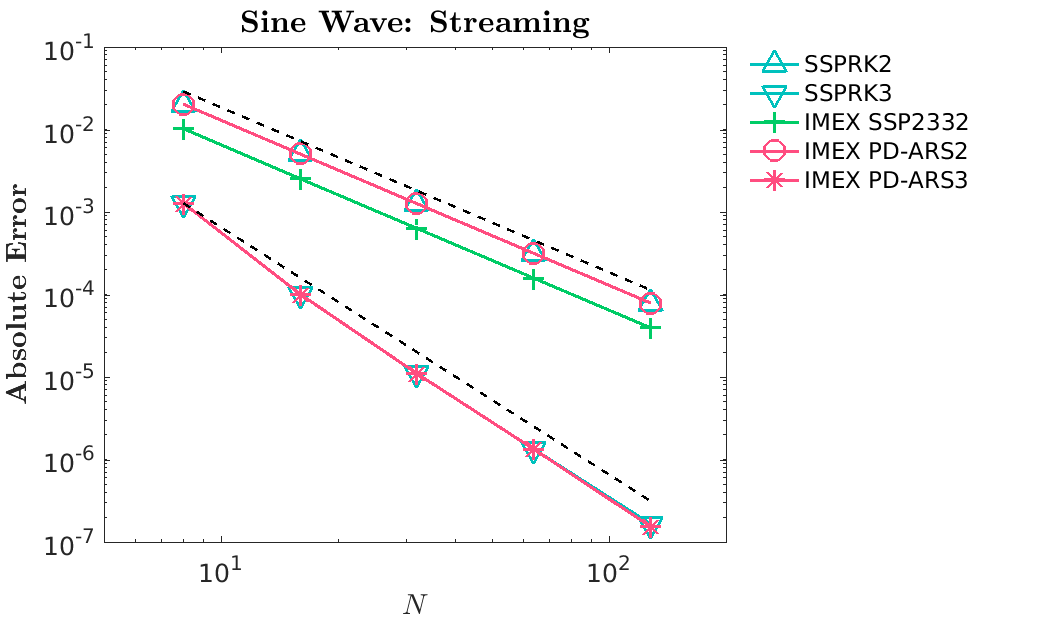
\includegraphics[width=0.8\textwidth]{figures/SineWaveStreaming}
   \caption{Absolute error versus number of elements $N$ for the streaming sine wave test.  Results employing various time stepping schemes are compared: SSPRK2 (cyan triangles pointing up), SSPRK3 (cyan triangles pointing down), SSP2332 (green crosses), PD-ARS with SSPRK2 (light red circles) and PD-ARS with SSPRK2 (light red hexagrams). Black dashed reference lines are proportional to $N^{-2}$ (top), and $N^{-3}$ (bottom), respectively.}
   \label{fig: SineWaveStreaming}
\end{figure}

\subsubsection{Sine Wave Damping}

This test, adapted from \cite{skinnerOstriker_2013}, is designed for absorption-dominated regimes, with $\sigma_{\Scatt} = 0$ and $f_0 = 0$, which results in exponential damping of the wave amplitude.
A periodic domain of unit length and initial condition $\cJ_{0} = \bcH_{0} = 0.5+0.49\times\sin\big(2\pi\,x\big)$ is used.
The amplitude of the analytical solution decreases as $e^{-\sigma_{\Ab} t}$.
For $\sigma_{\Ab}$ = 0.1, 1 and 10 we evolve the test until the initial condition has been damped by a factor $e^{-10}$. 
Figure~\ref{fig:SineWaveDamping} shows convergence results of the sine wave damping test in the relative error.
SSP2332, a second-order scheme, displays second-order convergence rate.  
The PD-ARS schemes are only first-order accurate.  
\begin{figure}[h]
  \centering
    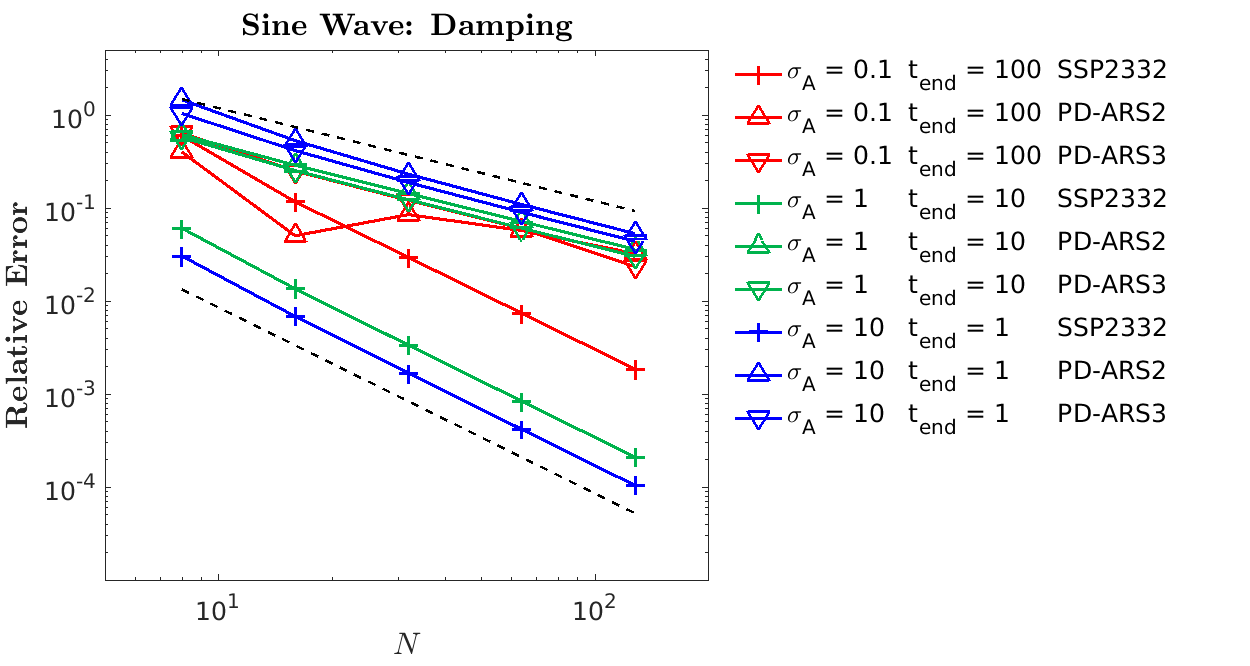
\includegraphics[width=0.9\textwidth]{figures/SineWaveDamping}
   \caption{Relative error versus number of elements, $N$, for the damping sine wave test. Results for different values of the absorption opacity $\sigma_{\Ab}$, employing various IMEX time stepping schemes, are compared.  Errors for $\sigma_{\Ab}=0.1$, $1$, and $10$ are plotted with red, green, and blue lines, respectively.  The IMEX schemes employed are SSP2332 ($+$), PD-ARS with SSPRK2 (circles) and PD-ARS with SSPRK3 (hexagram).  Black dashed reference lines are proportional to $N^{-1}$ (top) and $N^{-2}$ (bottom), respectively.}
  \label{fig:SineWaveDamping}
\end{figure}

\subsubsection{Sine Wave Diffusion}

The last test with known smooth solution, adopted from \cite{radice_etal_2013}, is the sine wave diffusion test, i.e. $\sigma_{\Ab} = 0$ and $f_0 = 0$.
A periodic domain $D=\{x:x\in[-3,3]\}$ with initial conditions $\cJ_{0} = 0.5+0.49\times\sin\big(\f{\pi\,x}{3}\big)$ and $\cH_{0} =-\f{1}{3\sigma_{\Scatt}}\pderiv{\cJ_{0}}{x}$ are used.  
The reference diffusion solution is given by $\cJ = \cJ_{0} \times \exp\big(-\f{\pi^2 t}{27\sigma_{\Scatt}}\big)$ and $\cH = (3\,\sigma_{\Scatt})^{-1}\pd{\cJ}{x}$.  
We evolve with $\sigma_{\Scatt}=10^{2}$, $10^{3}$, and $10^{4}$, and adjust the end time so that $t_{\mbox{\tiny end}}/\sigma_{\Scatt}=1$. 
Then the amplitude of the sine wave has been reduced by a factor $e^{-\pi^{2}/27}\approx0.694$ for all values of $\sigma_{\Scatt}$. 
Figure~\ref{fig:SineWaveDiffusionJ} shows the error versus $N$.  
SSP2332 and PD-ARS schemes display third-order accuracy for the number density, $\cJ$, and second-order accuracy for $\cH_{x}$, and their errors are difficult to distinguish.
PD-ARS with SSPRK2 behaves as good as SSP2332 in the diffusion region but requires one less implicit solves per time step.  

\begin{figure}[h]
  \centering
  \centerline{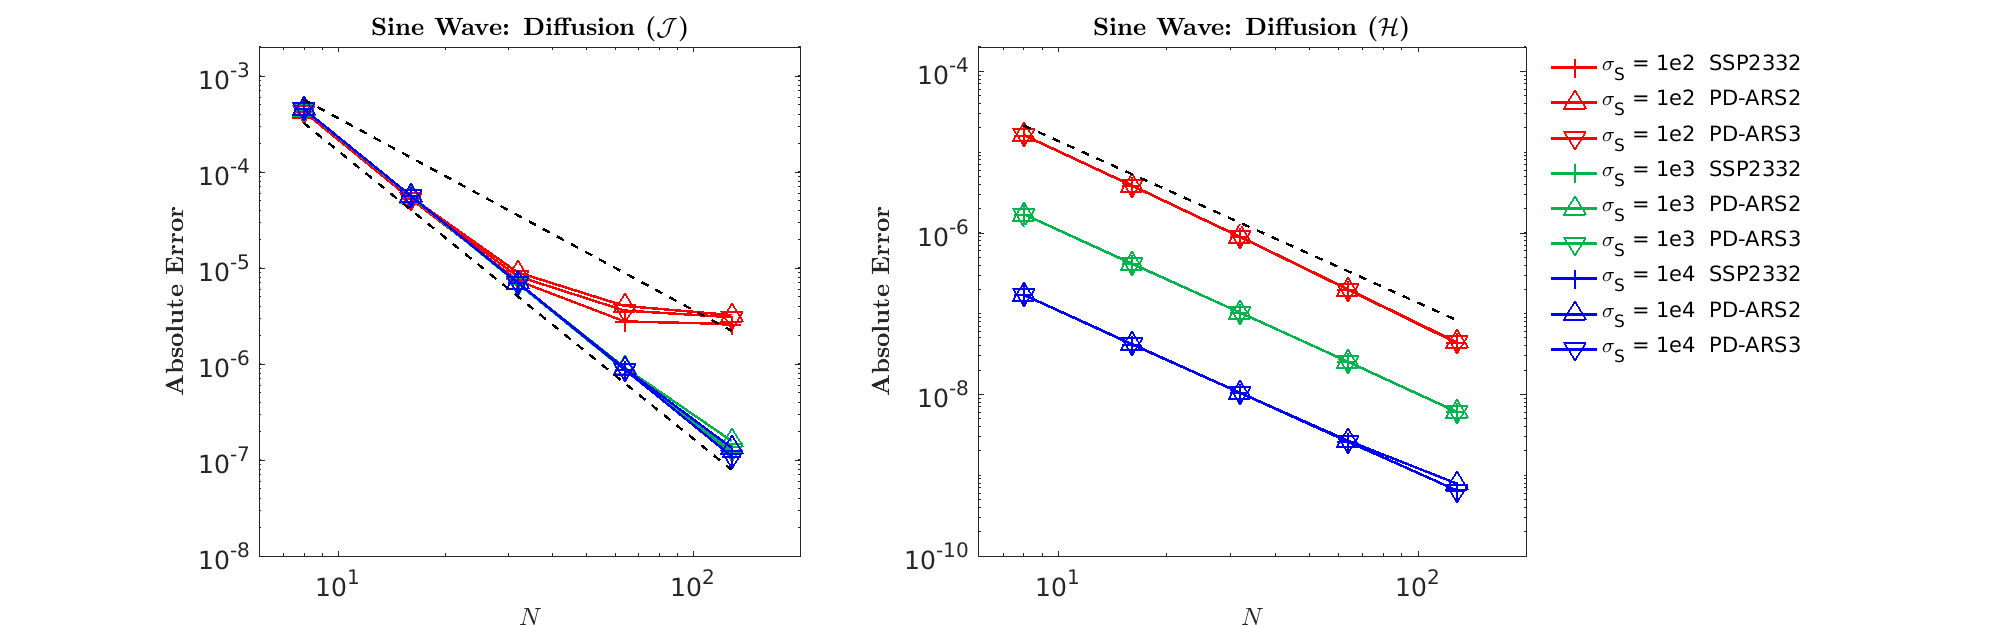
\includegraphics[width=1.2\textwidth]{figures/SineWaveDiffusion}}
   \caption{Absolute error for the number density $\cJ$ (left) and the number flux $\cH_{x}$ (right) versus number of elements for the sine wave diffusion test.  Results with different values of the scattering opacity $\sigma_{\Scatt}$, employing different IMEX schemes, are compared.  Errors with $\sigma_{\Scatt}=10^{2}$, $10^{3}$, and $10^{4}$ are plotted with red, green, and blue lines, respectively.  The IMEX schemes employed are:  SSP2332 ($+$), PD-ARS with SSPRK2 (circles), and PD-ARS with SSPRK3 (hexagram). Black dashed lines in the left plot are reference lines proportional to $N^{-2}$ (top) and $N^{-3}$ (bottom), respectively. Black dashed line in the right plot is a reference line proportional to $N^{-2}$ .}
   \label{fig:SineWaveDiffusionJ}
\end{figure}

\subsection{Neutrino Stationary State Test} \label{se: Neutrino Stationary State Test}

In this section we consider a more ``realistic'' test: two-dimensional multigroup neutrino transport with emission, absorption, and elastic scattering through a stationary background.  
This test is designed to test the realizability-preserving properties of the PD-ARS schemes.  
Figure~\ref{fig:NeutrinoStationaryTestEOS} plots the thermal state and the opacities used (adopted from \cite{Bruenn_1985}).  
This test is computed on a two-dimensional domain $D=\{\vect{x}\in\bbR^{2}:x^{1}\in[0,200], x^{2}\in[0,200]\}$ with a grid of 128 elements in each direction, a reflecting inner boundary and a homogeneous out-flowing outer boundary.
We use 10 energy groups to cover the range from 0~MeV to 300~MeV and initialize the neutrino number density to $\cJ = 10^{-99}$, flux density $\bcH=0$, and evolve until an approximate steady state is reached ($t=5$~ms).  
For this test, we employed the CB closure.  
We attempted to run this test with our PD-ARS schemes, SSP2332 from \cite{pareschiRusso_2005}, IMEXRKCB2 proposed by Cavaglieri \& Bewley \cite{cavaglieriBewley2015}, and the scheme proposed by McClarren et al. \cite{mcclarren_etal_2008}.
Only the PD-ARS schemes produce realizable moments and are able to evolve to a steady state.
The other schemes crashed after a few steps, when moments became non-realizable and the closure procedure failed.  

Results obtained with the PD-ARS IMEX schemes are plotted in Figure~\ref{fig:NeutrinoStationaryTestEvolve} for various times: $t=0.01$~ms (top panels), 0.35~ms (middle panels), and 5.0~ms (bottom panels).  
In the left column we plot the solution in the $|\vect{\cH}|\cJ$-plane.  
In the middle column we show scatter plots of the number density $\cJ$ versus radius for select neutrino energies: 5~MeV (red lines), 16~MeV (magenta lines), and $93$~MeV (blue lines).  
In the right column we plot the flux factor $|\vect{\cH}|/\cJ$ versus radius for the same neutrino energies as in the middle column.  
In the left panels, each solution point in the domain is marked as a red dot in the $|\vect{\cH}|\cJ$-plane, and the realizable domain is shown as the light blue region.  
The figures show that all the states in the simulation with the PD-ARS schemes are realizable.  

\begin{figure}[h]
  \centering
  \begin{tabular}{cc}
    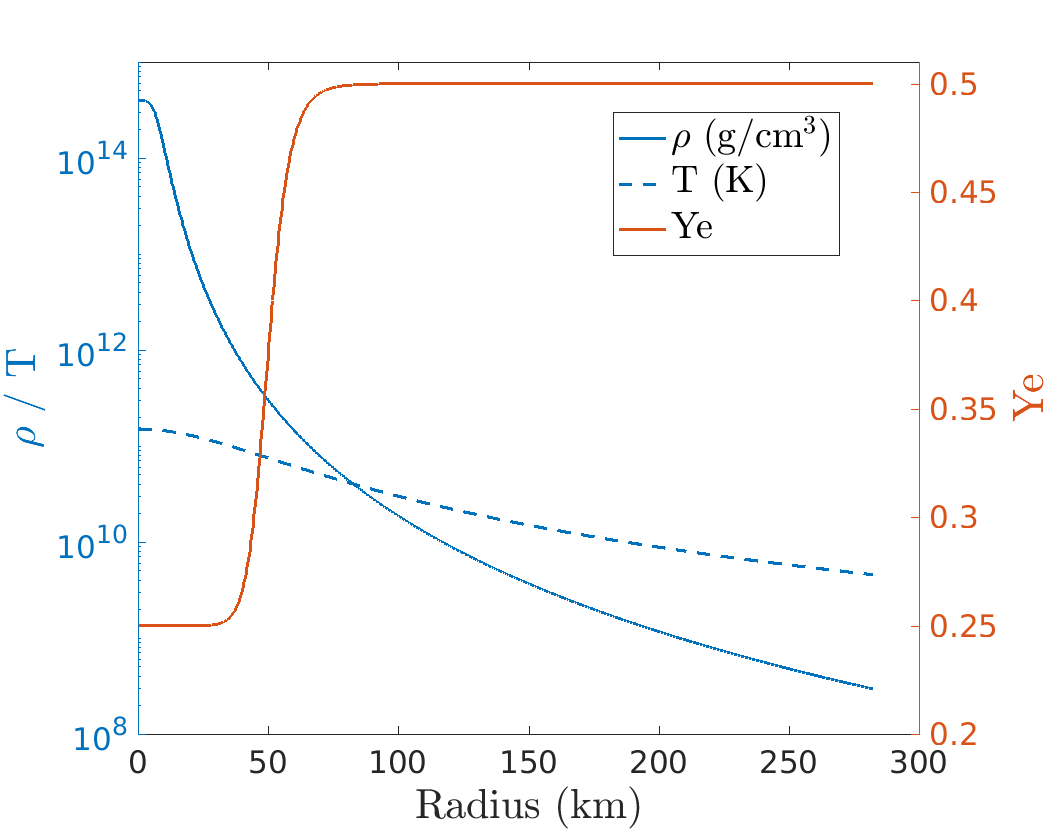
\includegraphics[width=0.45\textwidth]{figures/NStatinaryS_EOS}
    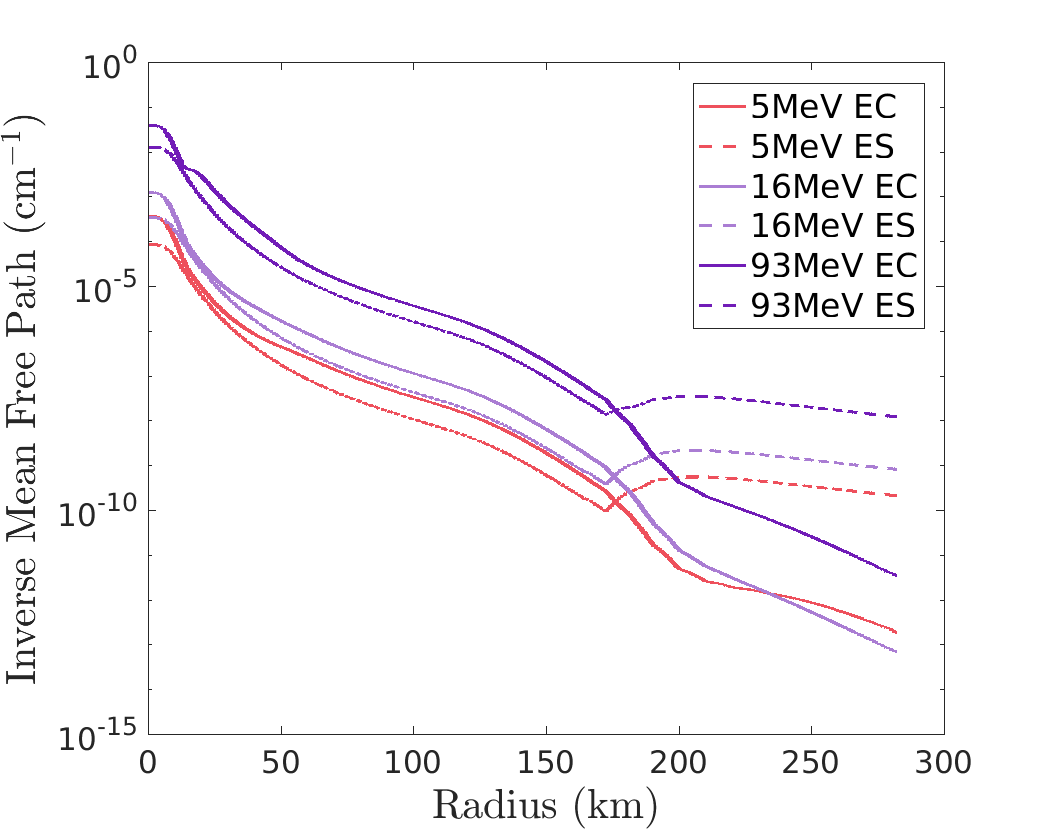
\includegraphics[width=0.45\textwidth]{figures/NSS_Opacities}
  \end{tabular}
   \caption{Left panel: thermal state of the background versus radius in the neutrino stationary state test; mass density (solid line), temperature (dashed line), and electron fraction (dotted line).  Right panel: corresponding opacities for select neutrino energies; absorptivity ($\sigma_{\Ab}$) and scattering opacity ($ \sigma_{\Scatt}$).}
   \label{fig:NeutrinoStationaryTestEOS}
\end{figure}

\begin{figure}[h]
  \centering
    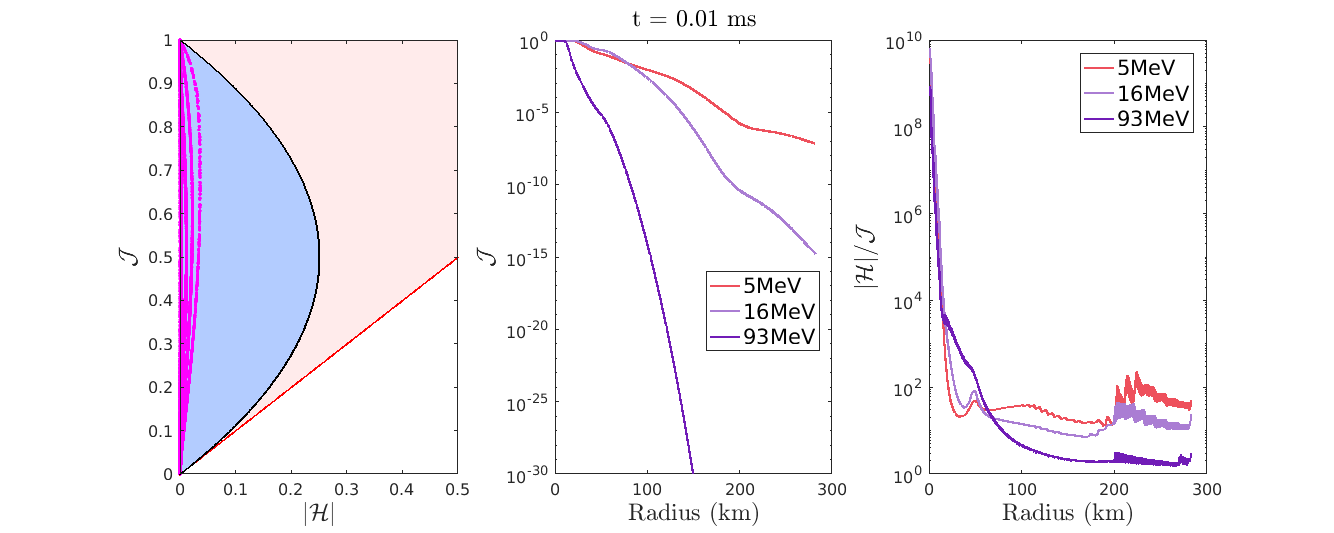
\includegraphics[width=\textwidth]{figures/NSS_1_1}\\
    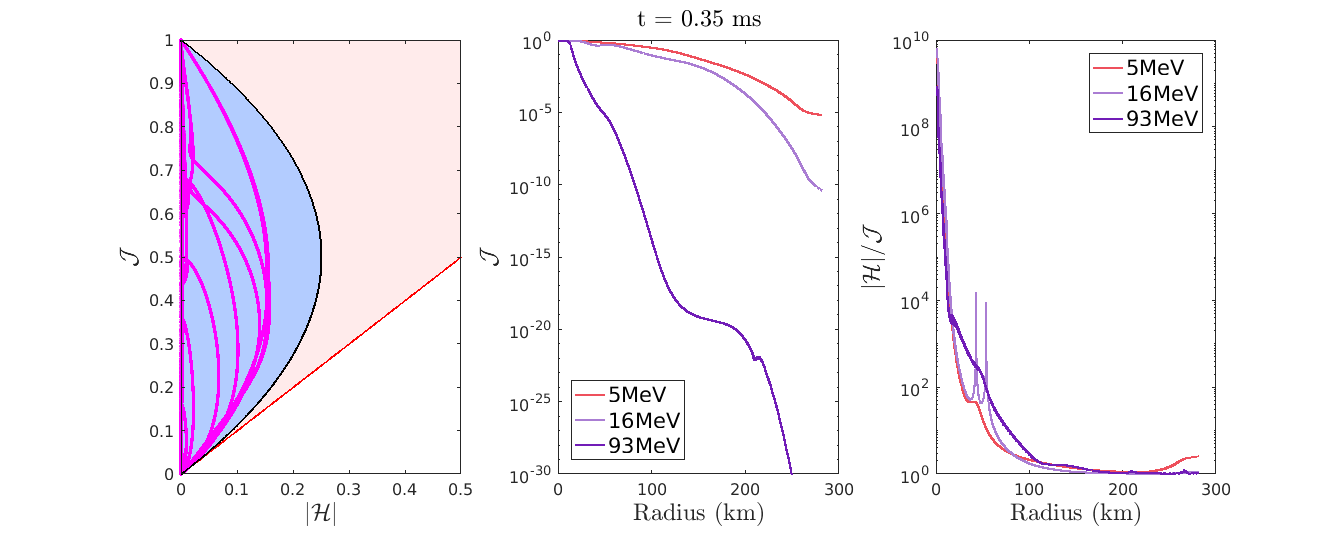
\includegraphics[width=\textwidth]{figures/NSS_3_1} \\
    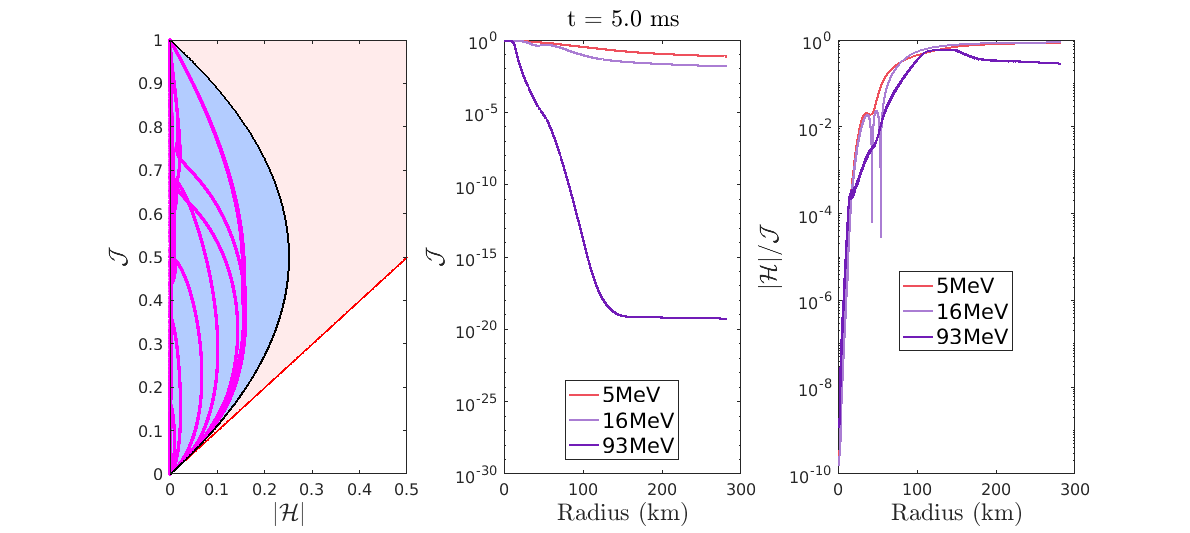
\includegraphics[width=\textwidth]{figures/NSS_5_1} \\
    \caption{Results from the neutrino stationary state test: moments relative to the realizable domain (left column, light blue domain is for $f \in [0,1]$ with black-solid-line as boundary, while light red is for $f\geq 0$ with thin-red-solid-line as boundary), the number density $\cJ$ versus radius (middle column), and the flux factor $|\bcH|/\cJ$ versus radius (right column), at $t = 0.01$~ms, 0.35~ms, and 5.0~ms.  For the plots in the left column, each $\bcM=(\cJ,\bcH)^{T}$ state is marked by a red dot, which are all inside the light blue region (the realizable domain for fermions).  The results of PD-ARS with SSPRK2 and PD-ARS with SSPRK3 are indistinguishable in these plots.}
    \label{fig:NeutrinoStationaryTestEvolve}
\end{figure}